\documentclass[12pt,a4paper,violet,oneside]{bbe}
\usepackage{blindtext}
\usepackage{hyperref}
\usepackage{amsthm}
\usepackage{cleveref,extpfeil,extarrows}
\usepackage{algorithm, algorithmicx,algpseudocode}
\usepackage[version=4]{mhchem}
\usepackage{ctex}
\renewcommand{\algorithmicrequire}{\textbf{Input:}} 
\renewcommand{\algorithmicensure}{\textbf{Output:}}
%\input{zhwinfonts}
\begin{document}
\setcounter{chapter}{3}
\chapter{贪心算法}
\section{贪心算法简介}
本章我们将介绍一种被称为\textbf{贪心算法}(greedy algorithm)的算法。贪心算法是一种\textbf{最优化算法},与先前介绍的分治算法不同:分治算法主要关注的是如何提升对一个\textbf{具有唯一确定解}的问题求解的效率,而贪心算法作为一种最优化算法,主要关注的是如何在一个\textbf{具有多个可行解}的问题中找出\textbf{具有最优值}的解,简称“\textbf{最优解}”。
\begin{remark}
对\textbf{最优解}这一概念可以作多种诠释,大多数情况下,如何定义“最优”其实是由问题本身解的结构与性质决定的,比如某问题的解是某一物品的数量$N$,那么最优解可能是指$N$的\textbf{最大值}或\textbf{最小值}。	
\end{remark}

通俗地说,贪心算法其实给出了这样一种策略来求取问题的最优解,它认为问题的最优解可由\textbf{原问题分解出的一系列子问题的最优解}(即\textbf{局部最优解})构成。更具体地说,使用贪心算法求取问题最优解时,会将原问题分为\textbf{多步}进行求解,每一步求解原问题的一部分,并\textbf{选择该步的最优解与已知的部分解合并},最终得到原问题的最优解。

但我们又不难看出,对一般性的问题而言,我们完全无法保证\textbf{局部最优解的组合一定是总体最优解},因此,\textbf{贪心算法只能适用于具有特定性质的最优化问题求解},一般来说,能够使用贪心算法求解的最优化问题,至少需要具有\textbf{贪心选择性}与\textbf{最优子结构}:
\begin{property}[\textbf{贪心选择性}]
	\textbf{贪心选择性}指:贪心算法每一步选择出的局部最优解一定是\textbf{原问题}的最优解的一部分。
\end{property}
\begin{property}[\textbf{最优子结构}]
	\textbf{最优子结构}指:贪心算法在每一步选择出局部最优解后,\textbf{已选择的局部最优解}与\textbf{剩余子问题的最优解}组合即为原问题的最优解。
\end{property}

我们可以从集合的角度对\textbf{贪心选择性}与\textbf{优化子结构}这两个性质作进一步理解,假设原问题的最优解为$A$,贪心算法在\textbf{有限步}内得到的局部最优解为$A_1,~A_2,\cdots,~A_n$,则\textbf{贪心选择性}保证了:
$$
\forall i,~1\leqslant i\leqslant n,~A_i\subseteq A\footnote{注意,此处$A_i\subseteq A$指的是每个$A_i$都可以找到原问题的某个最优解使之包含其中,而不是存在原问题的一个最优解使所有$A_i$均包含其中}
$$

\textbf{优化子结构}保证了:
$$
\forall i,~1\leqslant i\leqslant n,~\left(\bigcup\limits_{1\leqslant k\leqslant i}A_k\right)\cup\text{best}(i)=A
$$

其中:$\text{best}(i)$指贪心算法经过$i$步后\textbf{剩余子问题的最优解}。

据此,我们即可说明\textbf{贪心选择性}与\textbf{优化子结构}这两个性质的必要性:\textbf{贪心选择性}其实保证了贪心算法求得的局部最优解至少会包含于原问题的最优解中,这保证了算法最基本的\textbf{有效性},即至少不会解出不在原问题最优解中的成分。\textbf{优化子结构}则保证了算法求解的\textbf{可持续性},它本质上体现了原问题最优解的一种“\textbf{可拆分性}”:即\textbf{从原问题最优解中除去若干子问题的局部最优解,剩余的部分也依然对应着剩余子问题的最优解}。这就使得我们可以通过不断调用算法求取局部最优解来不断缩小剩余未求解的子问题的规模,直至\textbf{剩余子问题的最优解也可被算法求取}。

\begin{remark}
	某种意义上,\textbf{贪心选择性}与\textbf{优化子结构}其实是呈\textbf{递进关系}的,\textbf{具有优化子结构的问题一般一定会具有贪心选择性},因为既然原问题的最优解是由局部最优解与剩余子问题的最优解构成的,那么局部最优解肯定是包含在原问题最优解中的。
	
	那么,我们为什么还要单独给出\textbf{贪心选择性}这一性质呢?这其实是为我们证明贪心算法的有效性提供思路:先证明贪心算法在每步得到的局部最优解包含于原问题最优解(\textbf{贪心选择性}),再证明\textbf{在此基础上},原问题最优解除去若干子问题的局部最优解,对应的仍是剩余子问题的最优解(\textbf{优化子结构})。
	
	而上述证明思路在实现证明时仍会遇到诸多困难,这主要是因为上述对\textbf{贪心选择性}与\textbf{优化子结构}的定义涉及到算法迭代调用的过程,而在实际的算法正确性分析中,注意到\textbf{子问题其实仅与原问题在问题规模上存在差异},我们常常使用以下思路证明贪心选择性与优化子结构:
	\begin{itemize}
		\item \textbf{贪心选择性}:证明对规模为$N$的问题$P(N)$,使用\textbf{一次}贪心策略得出的局部最优解$a(N)$一定包含于$P(N)$的某一最优解$A(N)$中:
		$$
		a(N)\subseteq A(N),~\forall N\in\mathbb{N}_+
		$$
	\item \textbf{优化子结构}:证明对规模为$N$的问题$P(N)$,使用\textbf{一次}贪心策略得出的局部最优解为$a(N)$,剩余子问题为$P(M)$,则:
	$$
	a(N)\cup A(M)=A(N),~\forall N\in\mathbb{N}_+
	$$
	
	上述证明思路中的\textbf{贪心选择性}与\textbf{优化子结构}与前文中的并不等价,但两者结合起来是等价的:在对原问题$P(N)$使用第一次贪心策略时,应用\textbf{优化子结构}可知局部最优解$a(N)$与剩余子问题$P(M)$的最优解$A(M)$可共同构成原问题的最优解$A(N)$,而以下,每对剩余子问题使用一次贪心策略,应用\textbf{优化子结构}可知局部最优解与分解出的\textbf{下一级子问题}的最优解共同构成\textbf{当前子问题}的最优解,应用\textbf{贪心选择性}可知得到的局部最优解一定包含于\textbf{当前子问题}的最优解,进而包含于\textbf{上一级子问题}的最优解$\cdots$最终包含于\textbf{原问题}的最优解,可用如下迭代过程表示:
	$$
	\begin{array}{cl}
		a(N)\cup A(M_1)= A(N)&\text{第1次调用}\\
		a(N)\cup (a(M_1)\cup A(M_2))=(a(N)\cup a(M_1))\cup A(M_2)= A(N)&\text{第2次调用}\\
		\cdots&\\
		(a(N)\cup a(M_1)\cup\cdots \cup a(M_m))\cup A(M_{m+1})= A(N)&\text{第m+1次调用}\\
		\cdots&\\
	\end{array}
	$$
	\end{itemize}
\end{remark}

综上,我们可给出贪心算法的基本设计步骤:
\begin{itemize}
	\item 证明问题具有\textbf{贪心选择性}与\textbf{优化子结构}。
	\item 根据问题的贪心选择性和优化子结构,通过\textbf{贪心归纳}构造原问题的最优解。
\end{itemize}

以下,我们将通过一些具体的问题展示贪心算法的设计与使用。
\section{贪心算法示例1:活动选择问题}
\begin{example}
	假定有一个$n$个\textbf{活动}(activity)的集合$S=\{a_1,~a_2,\cdots,~a_n\}$,这些活动共用同一个资源,而该资源在某个时刻仅能供一个活动使用。对每个活动$a_i$,存在对应的\textbf{开始时间}$s_i$于\textbf{结束时间}$f_i$,活动$a_i$发生于$[s_i,~f_i)$中,若$a_i,~a_j$满足:$[s_i,~f_i)\cap[s_j,~f_j)=\varnothing$,则称$a_i$与$a_j$是\textbf{兼容的},我们希望选出一个\textbf{最大兼容活动集合},使得其中包含的活动个数最大。
	
	另外,我们不妨假设成立:
	$$
	f_1\leqslant f_2\leqslant\cdots\leqslant f_n
	$$
\end{example}

首先,我们不妨将问题一般化,我们记$S_{ij}$为\textbf{在$a_i$结束后开始,且在$a_j$开始前结束的活动构成的集合},并针对该集合,记$c[i,j]$为$S_{ij}$中包含的\textbf{最大兼容活动集合$A_{ij}$的元素个数}。以下,我们在$S_{ij}$上考查活动选择问题:

那么,我们应当如何设计\textbf{贪心策略}呢?注意到,我们如果希望$S_{ij}$的兼容活动集合元素个数尽可能大,则\textbf{每一个活动应当尽可能早地结束,方便后续活动的展开},于是我们设计贪心策略如下:\textbf{每次选取一个活动,且保证该活动是与先前已选取活动兼容的活动中结束时间最早的一个}。

比如,对$S_{ij}$,我们第一次选取的就是$S_{ij}$中结束时间最早的活动$a_k$,第二次则选取$S_{ij}-\{a_k\}$中与$a_k$兼容且结束时间最早的活动$\cdots$以此类推。以下,我们首先证明原问题\textbf{在这种贪心策略下}具有\textbf{贪心选择性}:
\begin{lemma}[\textbf{贪心选择性}]
	对任一子问题$S_k$,设$a_m$是$S_k$中结束时间最早的的活动,则$a_m$一定在$S_k$的\textbf{某个}(可能不唯一)最大兼容活动集合中。
\end{lemma}

\begin{proof}
	假定$A_k$为$S_k$的一个最大兼容活动集合,其中$a_j$为$A_k$中结束时间最早的活动。若$a_j=a_m$,则证明完成;若$a_j\ne a_m$,则令$A'_k=A_k-\{a_j\}+\{a_m\}$,由于$a_j$与$A_k-\{a_j\}$中的活动兼容,且$A_k-\{a_j\}$中的活动均在$a_j$后进行,$a_m$又是$S_k$中结束时间最早的活动,因此一定与$A_k-\{a_j\}$中的活动兼容,因此$A'_k$也是一个\textbf{最大兼容活动集合},证毕\footnote{这种基于一个最优解,通过局部最优解的替换构造另一个最优解的技巧是一种常见的证明方法,又被称为“\textbf{剪切-粘贴法}”}。
\end{proof}

在证明贪心选择性后,我们可以对原贪心策略进行进一步细化,当我们选取$S_{ij}$中结束时间最早的活动$a_k$后,不难得出$S_{ij}-\{a_k\}$中与$a_k$兼容的活动\textbf{要么在$a_k$开始前结束,要么在$a_k$结束后开始},因此与$a_k$兼容的活动集合即为$S_{ik}\cup S_{kj}$,而$S_{ik}$与$S_{kj}$即对应着我们需要求解的2个\textbf{子问题}。以下,我们将证明原问题具有\textbf{优化子结构}:
\begin{lemma}[\textbf{优化子结构}]
	若$S_{ij}$中结束时间最早的活动为$a_k$,则成立:
	$$
	A_{ij}=A_{ik}\cup\{a_k\}\cup A_{kj}
	$$
	
	其中$A_{ij},~A_{ik},~A_{kj}$均指\textbf{某个}最大兼容活动集合\footnote{其实我们不难发现$S_{ik}=\varnothing$,因为$a_k$为$S_{ij}$中结束时间最早的活动,则说明$a_k$为\textbf{下标最小}的活动(因为结束时间按下标顺序递增),因此若存在$a_s\in S_{ik}\subseteq S_{ij}$,则$s<k$,矛盾!因此最终只会分解为\textbf{1个子问题}}。
\end{lemma}

\begin{proof}
	由\textbf{贪心选择性}可知,一定存在$S_{ij}$的某个最大兼容活动集合$A_{ij}$使得$a_k\in A_{ij}$,以下我们证明可找到$S_{ik},~S_{kj}$的某个最大兼容活动集合$A_{ik},~A_{kj}$,使得:
	$$
		A_{ij}=A_{ik}\cup\{a_k\}\cup A_{kj}
	$$
	
	事实上,我们任取$S_{ik},~S_{kj}$的某个最大兼容活动集合$A_{ik},~A_{kj}$,$A_{ik}\cup\{a_k\}\cup A_{kj}$都是$S_{ij}$的最大兼容活动集合,这是因为$A_{ij}-\{a_k\}$中的元素要么在$S_{ik}$中,要么在$S_{kj}$中,因此:
	$$
	|A_{ij}|\leqslant|A_{ik}|+|A_{kj}|+1
	$$
	
	而$A_{ik}\cup\{a_k\}\cup A_{kj}$中的元素又是\textbf{互相兼容}的,因此$|A_{ij}|\geqslant|A_{ik}|+|A_{kj}|+1$,进而$|A_{ij}|=|A_{ik}|+|A_{kj}|+1$,证毕。

\end{proof}

\begin{remark}
	注意,我们无法直接证明原问题的\textbf{贪心选择性}与\textbf{优化子结构},因为这两者与算法所选取的\textbf{贪心策略}相关。因此,我们需要先确定算法所采用的贪心策略,再对贪心选择性与优化子结构进行\textbf{具化}并予以证明。
\end{remark}

综上,我们给出活动选择问题的算法设计,如\cref{alo4.1}所示:
\\
\begin{algorithm}[H]
	\caption{RECURSIVE-ACTIVITY-SELECTOR($s$,~$f$,~$k$,~$n$)}
	\label{alo4.1}
	\begin{algorithmic}[1] 
		\Require 活动起始时间集合$s$与结束时间集合$f$,活动集合$S{kn}$(对应参数$k,~n$)
		\Ensure $S_{kn}$中的\textbf{最大兼容活动集合}\textcolor{blue}{\Comment{定义结束时间$f_0=0$的虚拟活动$a_0$,对原问题调用RECURSIVE-ACTIVITY-SELECTOR($s$,~$f$,~0,~$n$)即可}}
		\State{$m=k+1$}
		\While{$m\leqslant n$~\textbf{and}~$s[m]<f[k]$}
		\State{$m=m+1$}\textcolor{blue}{\Comment{找在$a_k$后开始的最早结束(下标最小)的活动}}
		\EndWhile
		\If{$m\leqslant n$}
		\State{\Return$\{a_m\}\cup$RECURSIVE-ACTIVITY-SELECTOR($s$,~$f$,~$m$,~$n$)}
		\Else
		\State{\Return$\varnothing$}
		\EndIf
	\end{algorithmic} 
\end{algorithm}

\section{贪心算法示例2:Huffman编码}
\begin{example}
	假设使用\textbf{前缀码}编码一个具有$n$个字符的字符集$C_n$,我们很显然可以通过构造一个具有$n$个\textbf{叶子结点}的\textbf{二叉树}$T_n$来给出一种可行的编码方案,其中各叶子结点分别对应$C_n$中的$n$个字符。
	
	若对$c\in C_n$,记$d_{T_n}(c)$为该字符对应叶子结点的\textbf{深度},$c.\text{freq}$为该字符出现的\textbf{频率},则称:
	$$
	B(T_n)=\sum\limits_{c\in C_n}c.\text{freq}\cdot d_{T_n}(c)
	$$
	
	为该种编码方案对应的\textbf{代价},我们希望寻找一种使代价$B(T_n)$\textbf{最小}的编码方案。
\end{example}

针对该问题,\textbf{Huffman}提出了一种十分经典的贪心算法设计(以下简称为\textbf{Huffman算法}),该算法得到的使代价最小的最优编码方案被称为\textbf{Huffman编码}。

Huffman编码的实现是熟知的,即\textbf{自底向上}地构造二叉树,从$n$个叶子结点$c_1,~c_2,\cdots,~c_n$开始,构造一个以freq为关键字的\textbf{最小优先队列},每次从队列中识别两个\textbf{最低频率}的对象构造其父结点,并将这两个对象出队,\textbf{父结点}的freq赋值为两个\textbf{子结点}的freq之和并入队$\cdots$以此类推,直至二叉树$T_n$构造完成。

以下,我们着手证明Huffman算法的正确性,同样需要证明\textbf{在上述贪心策略下},原问题具有\textbf{贪心选择性}与\textbf{优化子结构}:
\begin{lemma}[\textbf{贪心选择性}]
	对规模为$n$的任一字符集$C_n$($n\in\mathbb{N}_+$),若$x,~y\in C_n$为$C_n$中\textbf{频率最小}的两个字符,则必存在一种最优编码方案,使得$x$与$y$的编码长度相同,且仅有\textbf{末尾位}互异\footnote{这实际上等价于认为$x,~y$具有共同的\textbf{父结点}}。
\end{lemma}
\begin{proof}
	我们同样采取“\textbf{剪切-粘贴法}”,任取一个最优编码方案对应的二叉树$T_n$,如果$x,~y$具有共同的父结点,则证明完成,以下我们考虑$x,~y$的父结点互异的情形:
	
	首先注意到,一个最优编码方案对应的二叉树一定是\textbf{满二叉树}\footnote{此处的满二叉树采用国外的定义:如果一棵二叉树的结点要么是叶子结点,要么它有两个子结点,则称其为\textbf{满二叉树}},因为若不是满二叉树,则代表存在\textbf{不是叶子结点且没有两个子结点}的结点,即仅存在一个子结点的结点,将该结点从树中删去,并将其子结点与其父结点相连,新生成的树仍对应一个二叉树,而对应编码的长度因树的深度减小而减小,进而导致该二叉树对应的编码方案的代价小于原二叉树对应的最优编码方案(此处默认字符出现的频率均为\textbf{正值}),矛盾!
	
	因此,我们总可找到深度\textbf{相同且最大}的叶子结点对应的字符$a,~b$,将其与$x,~y$替换,则注意到:
	$$
	x.\text{freq},~y.\text{freq}\leqslant a.\text{freq},~b.\text{freq}
	$$
	$$
	d_{T_n}(a)=d_{T_n}(b)>d_{T_n}(x),~d_{T_n}(y)
	$$
	
	而在交换结点后的二叉树$T_n'$中,成立:
	$$
	d_{T_n'}(a),~d_{T_n'}(b)<d_{T_n'}(x)=d_{T_n'}(y)
	$$
	
	以及:
	$$
	\{d_{T_n'}(a),~d_{T_n'}(b)\}=\{d_{T_n}(x),~d_{T_n}(y)\},~d_{T_n'}(x)=d_{T_n'}(y)=d_{T_n}(a)=d_{T_n}(b)
	$$
	因此:
	$$
	\begin{array}{rl}
		B(T_n')-B(T_n)&=(d_{T_n'}(a)-d_{T_n}(a))a.\text{freq}+(d_{T_n'}(b)-d_{T_n}(b))b.\text{freq}\\
		&~~~~+(d_{T_n'}(x)-d_{T_n}(x))x.\text{freq}+(d_{T_n'}(y)-d_{T_n}(y))y.\text{freq}\\
		&=(d_{T_n'}(a)-d_{T_n}(a))a.\text{freq}+(d_{T_n'}(b)-d_{T_n}(b))b.\text{freq}\\
		&~~~~+(d_{T_n}(a)-d_{T_n}(x))x.\text{freq}+(d_{T_n}(b)-d_{T_n}(y))y.\text{freq}\\
		&\leqslant(d_{T_n'}(a)-d_{T_n}(x))a.\text{freq}+(d_{T_n'}(b)-d_{T_n}(y))b.\text{freq}\\
		&\leqslant(d_{T_n'}(a)+d_{T_n'}(b)-d_{T_n}(x)-d_{T_n}(y))\cdot\max\{a.\text{freq},~b.\text{freq}\}=0
	\end{array}
	$$
	
	因此$B(T_n')\leqslant B(T_n)$,又由$B(T_n)$最小,可得$B(T_n')=B(T_n)$,故$T_n'$也对应着一种最优编码方案,证毕。
\end{proof}

\begin{lemma}[\textbf{优化子结构}]
	对规模为$n$的任一字符集$C_n$($n\in\mathbb{N}_+$),若$x,~y\in C_n$为$C_n$中\textbf{频率最小}的两个字符,则定义新字符$z$,满足:
	$$
	z.\text{freq}=x.\text{freq}+y.\text{freq}
	$$
	
	并令$C_{n-1}=C_n-\{x,~y\}+\{z\}$,令$T_{n-1}$为$C_{n-1}$最优编码方案对应的二叉树,并将$T_{n-1}$中对应$z$的叶子结点替换为一个以$x,~y$为叶子结点的内部结点,得到树$T_n$,则$T_n$对应的编码方案为$C_n$的最优编码方案。
\end{lemma}
\begin{proof}
	易于验证$T_n$为二叉树,且除$x,~y$外,其余字符对应的编码长度不变,同时有:
	$$
	\begin{array}{rl}
		B(T_n)-B(T_{n-1})&=d_{T_n}(x)x.\text{freq}+d_{T_n}(y)y.\text{freq}-d_{T_{n-1}}(z)z.\text{freq}\\
		&=(d_{T_n}(x)-d_{T_{n-1}}(z))x.\text{freq}+(d_{T_n}(y)-d_{T_{n-1}}(z))y.\text{freq}\\
		&=x.\text{freq}+y.\text{freq}
	\end{array}
	$$
	
	因此有:
	$$
	B(T_{n-1})=B(T_n)-x.\text{freq}-y.\text{freq}
	$$
	
	以下使用\textbf{反证法},假设$T_n$对应的编码方案不是最优的,则存在$T_{n}'$对应最优编码方案,将$T_n'$中的$x,~y$结点删去,并将其父结点命名为$z$,使$z.\text{freq}=x.\text{freq}+y.\text{freq}$,得到二叉树$T_{n-1}'$,$T_{n-1}'$显然也对应着$C_{n-1}$的一种编码方案,但是:
	$$
	B(T_{n-1}')=B(T_n')-x.\text{freq}-y.\text{freq}<B(T_n)-x.\text{freq}-y.\text{freq}=B(T_{n-1})
	$$
	
	这与$B(T_{n-1})$最小矛盾!故$T_n$对应的编码方案为$C_n$的最优编码方案,证毕。
\end{proof}
\section{贪心算法示例3:最小生成树问题}
\begin{example}
	给定\textbf{无向连通图}$G=(V,~E)$,对$\forall (u,~v)\in E$给定权重函数$w(u,~v)$,寻找无环子集$T\subseteq E$,使得$T$可将所有$v\in V$连接起来,且使$w(T)=\sum\limits_{(u,~v)\in T}w(u,~v)$最小,由于$T$是无环的且连接所有结点,因此$T$必定是一棵树,称为图$G$的\textbf{最小生成树}。
\end{example}


有两个非常经典的贪心算法设计用于求解最小生成树问题:\textbf{Kruscal算法}与\textbf{Prim算法},在离散数学课程中已对这两种算法的正确性进行证明,此处不再赘述,仅对算法实现进行简要说明:

\textbf{Kruscal算法}的主要思路是:每次都在图$G$中寻找权重最小的边$(u,~v)$,判断子集$T$加入$(u,~v)$后是否仍为树,若为树,则$T=T+\{(u,~v)\}$;若不为树,则$T$保持不变,继续寻找剩余边中权重最小的边$\cdots$以此类推,直至无边可继续加入,此时得到的子集$T$即为图$G$对应的\textbf{最小生成树}。

虽然可以证明,利用上述描述的思路可以找出最小生成树$T$,但其却不利于算法实现,因为这种思路中的一些操作的实现比较复杂,比如:\textbf{判断一个子集$T$是否为树}等。如果单纯按照上述思路实现算法,算法对应的复杂度也是很不可观的。因此,我们常采用以下的等价思路实现算法:

在初始状态时,将$G$中的每个结点都视为一个\textbf{树}进行存储,同时,将$G$的边集$E$内的元素按\textbf{权重从小到大}的顺序排列,以下,按顺序取出边集$E$内的边$(u,~v)$,判断结点$u,~v$是否位于\textbf{同一棵树}上,若是,则无操作\footnote{因为此时若将$(u,~v)$加入子集$T$中,一定会在$T$中生成\textbf{环}},若否,则令子集$T$加入边$(u,~v)$,并将结点$u,~v$所在的树合并为一棵树$\cdots$以此类推,直至无边可继续操作,此时得到的子集$T$即为图$G$对应的\textbf{最小生成树}。该思路对应的伪代码实现如\cref{alo4.2}所示:
\\
\begin{algorithm}[H]
	\caption{MST-KRUSCAL($G$,~$w$)}
	\label{alo4.2}
	\begin{algorithmic}[1] 
		\Require 无向连通图$G(V,~E)$,边集$E$元素的权重集合$w$
		\Ensure 图$G$的最小生成树$T$
		\State{$T=\varnothing$;}\textcolor{blue}{\Comment{初始化最小生成树}}
		\ForAll{$v\in G.V$}
		\State{MAKE-SET($v$);}\textcolor{blue}{\Comment{对每个结点建树}}
		\EndFor
		\State{Sort $(u,~v)\in G.E$ in increasing order by $w(u,~v)$;}
		\For{$(u,~v)\in G.E$ in increasing order by $w(u,~v)$}
		\If{FIND-SET($u$)$\ne$FIND-SET($v$)}\textcolor{blue}{\Comment{如果$u$与$v$不在一棵树上}}
		\State{$T=T\cup\{(u,~v)\}$,~UNION($u$,~$v$);}\textcolor{blue}{\Comment{合并$u$与$v$所在树}}
		\EndIf
		\EndFor
		\State{\Return$T$;}
	\end{algorithmic} 
\end{algorithm}
\begin{remark}
	Kruscal算法的时间复杂度受诸多因素影响,一般可表示为$O(E\log E)$或$O(E\log V)$。
\end{remark}
\begin{algorithm}[H]
	\caption{MST-PRIM($G$,~$w$,~$r$)}
	\label{alo4.3}
	\begin{algorithmic}[1] 
		\Require 无向连通图$G(V,~E)$,边集$E$元素的权重集合$w$,最小生成树的根结点$r$
		\Ensure 图$G$的最小生成树$T$
		\ForAll{$u\in G.V$}
		\State{$u.\text{key}=\infty$,~$u.\pi=\text{NIL}$;}
		\EndFor
		\State{$r.\text{key}=0$,~$Q=G.V$;}\textcolor{blue}{\Comment{根结点$\text{key}$值设为0,同时构建最小优先队列}}
		\While{$Q\ne \varnothing$}
		\State{$u=$EXTRACT-MIN($Q$);}\textcolor{blue}{\Comment{取出队首元素加入$T$}}
		\ForAll{$v\in G.Adj[u]$}\textcolor{blue}{\Comment{考虑$u$的所有相邻结点}}
		\If{$v\in Q$ \textbf{and} $w(u,~v)<v.\text{key}$}
		\State{$v.\pi=u$,~$v.\text{key}=w(u,~v)$;}
		\EndIf
		\EndFor
		\EndWhile
		\State{\Return$\{(v,~v.\pi)|v\in V-\{r\}\}$;}
	\end{algorithmic} 
\end{algorithm}

\textbf{Prim算法}的主要思路是:首先任取$G$中的某一结点$r$作为最小生成树$T$的\textbf{根结点},其次,每次在连接$T$与$G-T$的所有边中选取\textbf{权重最小}的边$(u,~v)$加入$T$(可以证明,此时$T$仍为树)$\cdots$以此类推,直至$T$包含$G$中所有结点,此时的$T$即为图$G$的最小生成树。

而在具体实现Prim算法时,我们可以对$\forall u\in G.V$定义两个关键字:$\text{key}$与$\pi$,其中$u.\text{key}$指\textbf{连接$u$与$T$中结点所有边中权重最小边对应的权重},在初始化时,除根结点$r$外的所有结点的$\text{key}$均被设置为$\infty$,因为此时$T$还未加入结点;$u.\pi$指当$u$在$T$中时,其对应的\textbf{父结点},在初始化时被设置为$\text{NIL}$,代表所有结点均无父结点。

以下,基于关键字$\text{key}$,构建结点的最小优先队列$Q$,则根结点$r$一定位于\textbf{队首},之后再循环令队首元素$u$出队,将其置入树$T$中,再对所有与队首元素$u$\textbf{相邻}且\textbf{未在$T$内}的结点$v$的$\pi$与$\text{key}$进行更新,具体更新原则为:如果$w(u,~v)<v.\text{key}$,代表$v$与$T$中结点所有边中的最小边需要更新为$(u,~v)$,对应$v.\text{key}$需要更新为$w(u,~v)$,同时当$v$加入$T$时,其父结点$v.\pi$也应更新为$u$。算法的具体实现如\cref{alo4.3}所示,最终得到的最小生成树应为:
$$
T=\{(v,~v.\pi)|v\in V-\{r\}\}
$$
\begin{remark}
	Kruscal算法的时间复杂度受建立最小优先队列的方式影响,一般可表示为$O(E\log V)$。
\end{remark}
\section{贪心算法示例4:单源最短路径问题}
\begin{example}
	给定有向图$G(V,~E)$以及对应的权重函数$w: E\to \mathbb{R}_+$,$w$将每条边映射至正实数权重值上。设给定路径$p=<v_0,~v_1,\cdots,~v_k>$的\textbf{权重}定义为:
	$$
	w(p)=\sum\limits_{i=1}^kw(v_{i-1},~v_i)
	$$
	
	同时,定义由结点$u$到结点$v$的\textbf{最短路径权重}$\delta(u,~v)$为:
	$$
	\delta(u,~v)=\left\{\begin{array}{lcl}
		\min\{w(p):~u\xrightarrow[]{p}v\}&&\text{如果存在从$u$到$v$的路径$p$}\\
		\infty&&\text{其他}
	\end{array}\right.
	$$
	
	\textbf{单源最短路径问题}需要求取从给定\textbf{源结点}$s\in V$到其余所有结点的\textbf{最短路径}。
\end{example}

\textbf{单源最短路径问题}有一个比较特殊的性质:我们事实上可以直接证明其具有\textbf{优化子结构},而无需考虑具体采用怎样的贪心策略,换言之,我们可以证明\textbf{对任意规模的单源最短路径问题,其包含的子问题的最优解一定也包含于原问题的最优解中},更进一步,我们可使用\hyperref[le4.1]{Lemma~4.5}进行描述:
\begin{lemma}[\textbf{优化子结构}]\label{le4.1}
	给定有向图$G(V,~E)$以及对应的权重函数$w: E\to \mathbb{R}_+$,设$p=<v_0,~v_1,\cdots,~v_k>$为从$v_0$到$v_k$的一条\textbf{最短路径},则对$\forall i,j,~0\leqslant i\leqslant j\leqslant k$,$p_{ij}=<v_i,~v_{i+1},\cdots,~v_j>$为从$v_0$到$v_k$的一条\textbf{最短路径}。
\end{lemma}
\begin{proof}
	记路径$p=p_{0i}+p_{ij}+p_{jk}$,则有:
	$$
	w(p)=w(p_{0i})+w(p_{ij})+w(p_{jk})
	$$
	
	采用反证法,若存在路径$p'_{ij}$使得$w(p'_{ij})<w(p_{ij})$,则构造从$v_0$到$v_k$的路径$p'=p_{0i}+p'_{ij}+p_{jk}$,有:
	$$
	w(p')=w(p_{0i})+w(p'_{ij})+w(p_{jk})<w(p_{0i})+w(p_{ij})+w(p_{jk})=w(p)
	$$
	
	这与$w(p)$的最小性矛盾!因此$p_{ij}$为从$v_0$到$v_k$的一条最短路径。
\end{proof}

在证明完问题具备优化子结构后,我们给出单源最短路径问题的一个经典贪心算法设计——\textbf{Dijkstra算法}。
\\
\begin{algorithm}[H]
	\caption{DIJKSTRA($G$,~$w$,~$s$)}
	\label{alo4.5}
	\begin{algorithmic}[1] 
		\Require 有向图$G(V,~E)$,权重函数$w$,源结点$s$
		\Ensure 以$s$为源结点的单源最短路径集合$S$
		\ForAll{$u\in G.V$}
		\State{$u.d=\infty$,~$u.\pi=\text{NIL}$;}
		\EndFor
		\State{$S=\varnothing$,~$s.d=0$,~$Q=G.V$;}\textcolor{blue}{\Comment{以$d$为关键字构建最小优先队列$Q$}}
		\While{$Q\ne \varnothing$}
		\State{$u=$EXTRACT-MIN($Q$),~$S=S\cup\{u\}$;}\textcolor{blue}{\Comment{$u$加入集合$S$}}
		\ForAll{$v\in G.Adj[u]$}
		\State{RELAX($u$,~$v$,~$w$);}\textcolor{blue}{\Comment{松弛操作}}
		\EndFor
		\EndWhile
		\State{\Return $S$;}
	\end{algorithmic} 
\end{algorithm}

在介绍Dijkstra算法前,同样需要先对相关概念进行预定义:我们使用集合$S$保存\textbf{已找到最短路径的结点},对结点$v$,我们同样定义两个关键字:$d$与$\pi$,$v.d$指的是由源结点$s$到结点$v$最短路径权重的\textbf{上界},一般也称为对最短路径权重的\textbf{估计};$v.\pi$指的是当由源结点$s$到结点$v$的路径权重取$v.d$时,结点$v$对应的\textbf{前驱结点}。

进而我们很容易有:
\begin{lemma}[\textbf{上界性质}]
	对于$\forall v\in G.V$,总成立:
	$$
	\delta(s,~v)\leqslant v.d
	$$
\end{lemma}

以下,我们需要引入对结点的\textbf{松弛操作},该操作可以用于更新结点$v$的$v.d$以及对应的$v.\pi$,松弛操作对应的伪代码如\cref{alo4.4}所示:
\\
\begin{algorithm}[H]
	\caption{RELAX($u$,~$v$,~$w$)}
	\label{alo4.4}
	\begin{algorithmic}[1] 
		\Require 结点$u,~v$,权重函数$w$\textcolor{blue}{\Comment{引入结点$u$对结点$v$进行\textbf{松弛操作}}}
		\If{$v.d>u.d+w(u,~v)$}
		\State{$v.d=u.d+w(u,~v)$;}
		\State{$v.\pi=u$;}
		\EndIf 
	\end{algorithmic} 
\end{algorithm}

松弛操作的思想非常朴实,即对结点$v$,如果我们能够找到一个结点$u$,满足$v.d>u.d+w(u,~v)$,则我们就可以取源结点$s$到结点$u$的路径权重取$u.d$对应的路径加入$(u,~v)$,得到一条源结点$s$到结点$v$,且路径权重为$u.d+w(u,~v)$的路径,进而可以对$v.d$以及$v.\pi$进行更新。

以下,我们便可以给出Dijkstra算法的具体实现:

\textbf{Dijkstra算法}给出的贪心策略如下:给定源结点$s\in V$,同时假设对$S\subseteq V$,$s$到$\forall v\in S$的最短路径都已被找到,以下考查$V-S$中\textbf{最短路径估计最小的结点}$u$,将$u$加入$S$,并基于结点$u$,对所有以$u$为\textbf{前驱}的结点$v$进行\textbf{松弛操作}。

进而我们可以尝试证明在这种贪心策略下,原问题具有\textbf{贪心选择性}:
\begin{lemma}[\textbf{贪心选择性}]\label{le4.2}
	对每个结点$u\in V$,当结点$u$被加入到集合$S$时,有$u.d=\delta(s,~u)$\footnote{一般地,在初始化时,我们会令源结点$s$的$s.d=0$,其余结点的$v.d=\infty$,另外对$\forall v\in G.V$(包括源结点),均令$v.\pi=\text{NIL}$}。
\end{lemma}
\begin{proof}
	\hyperref[le4.2]{Lemma~4.7}实际上需要证明一个\textbf{循环不变式},即对每次循环取出结点$u$加入集合$S$的操作进行考查,为此我们需要分别考虑循环开始、保持与终止时\hyperref[le4.2]{Lemma~4.7}的正确性。
	
	循环开始时$S=\varnothing$,第一个被加入的结点就是\textbf{源结点}$s$,显然成立。
	
	在循环过程中,我们采用反证法证明\hyperref[le4.2]{Lemma~4.7},假设存在结点$u$使得$u$加入集合$S$后,$u.d\ne \delta(s,~u)$,则必有$u.d>\delta(s,~u)$,假设$u$是第一个满足$u.d>\delta(s,~u)$的结点,又由$s.d=\delta(s,~s)=0$,可知$u$不可能为$s$,这也就意味着$u$在加入集合$S$前,集合$S$就已非空。
	
	同时,又一定存在由源结点$s$到$u$的路径,否则$u.d=\delta(s,~u)=\infty$,矛盾!而既然存在路径,便必存在由$s$至$u$的\textbf{最短路径}$p$(因为路径总数有限)。
	\begin{figure}[!htbp]
		\centering
		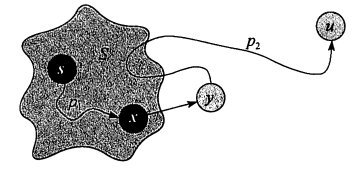
\includegraphics[width=0.4\textwidth]{fig4.1}
		\caption{最短路径$p$示意图}
		\label{fig4.1}
	\end{figure}

如\cref{fig4.1}所示,考查将$u$加入前的集合$S$,则路径$p$中应当可以找到一个结点$y$,使得$y\in V-S$但$y$的前驱$x\in S$,我们记路径$p$中\textbf{由$s$至$x$的一段}为$p_1$,\textbf{由$y$至$u$的一段}为$p_2$\footnote{当然,$p_1,~p_2$可能不包含任何结点,此时对应的是$x=s,~y=u$的情形},于是有:
$$
p:~s\xrightarrow[]{~p_1~}x\to y\xrightarrow[]{~p_2~}u
$$

由于在将结点$x$加入$S$时,会基于$x$对$y$进行\textbf{松弛操作},因此有:
$$
y.d\leqslant x.d+w(x,~y)=\delta(s,~x)+w(x,~y)
$$

此处的“$\leqslant$”是由于$y.d$可能本身就不超过$x.d+w(x,~y)$,进而无需进行操作,同时注意到$\delta(s,~x)+w(x,~y)$为最短路径的一条子路径的权重,利用\hyperref[le4.1]{Lemma~4.5},可知$\delta(s,~x)+w(x,~y)=\delta(s,~y)$,进而$y.d=\delta(s,~y)$(\textbf{上界性质})。

同时我们注意到:
$$
y.d=\delta(s,~y)\leqslant\delta(s,~u)\leqslant u.d
$$

但我们当前考虑的是结点$u$加入集合$S$前的情形,换言之,我们已知在下一循环内是结点$u$加入集合$S$,因此必有$u.d\leqslant y.d$,进而有$y.d=u.d$。

进而$y.d=u.d=\delta(s,~u)$,这与假设$u.d>\delta(s,~u)$矛盾!故\hyperref[le4.2]{Lemma~4.7}成立。

在算法终止时,所有结点均被加入$S$中,因此对$\forall u\in V$,当$u$被加入到集合$S$时,有$u.d=\delta(s,~u)$,证毕。
\end{proof}

综上,我们完成了对Dijkstra算法的正确性分析,算法对应的伪代码如\cref{alo4.5}所示。
	%\blinddocument
\end{document}
